\section{第三类:投射阴影多边形}
在第一类和第二类算法中,阴影可以定义成边在表面上的投影。
也可以定义成它们包围的空间体积。
通过将物体的表面加进数据中,最后一类的阴影算法在隐藏表面计算中包含了阴影体积值。
假设一个多边形物体,通过由轮廓边和光源位置确定的平面,可以给定阴影表面。
每条这样的边确定了一个多边形,它的边界就是这条边。
这两条边是由光源位置,边的出射点和视场的边界确定的(图\ref{fig:fig4})。
\begin{figure*}[h]
\centering
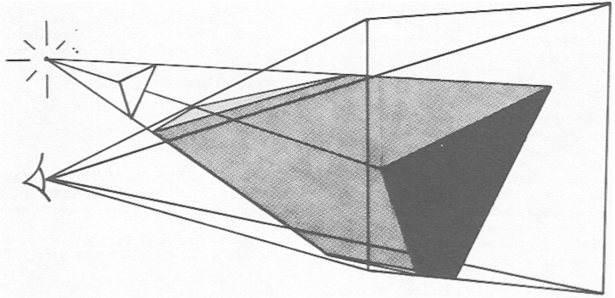
\includegraphics[width=0.9\linewidth]{fig4}
\caption[fig4]{按视场裁剪的阴影多边形}
\label{fig:fig4}
\end{figure*}
必须保持这个多边形的辨识,这样一个阴影体积(正面多边形)的近表面才能从远表面(背面多边形)中区分出来。
所以面向光源的多边形,加上一个物体的投射阴影多边形的集合,共同确定了该物体的阴影体积。\\
当应用一个扫描隐藏表面算法时,阴影多边形可以就像其他数据那样处理。
只有可见表面的阴影才需要不同的处理方式。
阴影多边形本身是不可见的,所以它们不用计入可见性的决定中。
但是,阴影表面的深度顺序和可见的表面决定了阴影。
一个正面阴影表面使任何之后的东西置于阴影中,而一个背面阴影表面取消了正面阴影表面的效果。
例如,一个桩子或者柱子可能投射一个包含单个多边形对的的阴影表面。
任何在这两个阴影多边形间的表面都会在阴影中,而在这两个多边形前面或者后面的表面则是正常地被遮盖。\\
如果最前面的阴影表面是背面的,那么任何在它前面的东西都在阴影中。
如果最后面的阴影表面是正面的,那么任何在它后面的东西都在阴影中。
当出射点在阴影中,或者表面在视场的很大一部分上投射了阴影了,这种情况就会出现。
所以,无论何时,只要表面在一个背面的最前阴影多边形之前,或者这个表面刺透的正面阴影多边形比背面阴影多边形多,那这个表面就在阴影中。
在一个可见表面和一个阴影多边形相交的地方,就会形成阴影边界。\\
为了处理阴影多边形,要对扫描隐藏表面算法进行调整,包含仅改变计算阴影的内循环。
可以用阴影多边形的两个性质来简化计算。
第一,阴影多边形是不可见的。
所以,只包含阴影多边形的扫描线可以被忽略。
第二,由轮廓边投影形成的阴影多边形不会和另一个相交(只要用的是单个光源)。
所以这些多边形的深度顺序是不变的。\\
使用Bouknight的扫描算法的变种(这种类型算法的详细描述可见\cite{4}\cite{12}),在y方向排序,x方面合并的步骤中,阴影多边形可以像其他多边形那样处理。
通常,扫描算法需要维护一个按深度排序的所有被扫描片段的列表,这些片段在扫描线上会被一束由当前位置出射点射出的光线穿透。
阴影多边形会频繁地导致相当长的扫描片段,大大地增加了一张图像的平均深度复杂度。
正如Sutherland等人\cite{12}指出的,深度复杂度的增加会严重阻碍扫描算法的表现。\\
但是,在产生扫描片段期间,阴影多边形只需在某些条件下考虑。
阴影多边形不会相交的事实允许有利地利用扫描线到扫描线的一致性。
随着扫描向图像下方移动,只有当新的多边形添加进来,或者旧的多边形被删除时,阴影多边形的深度顺序才会改变。
所以重建和更新阴影多边形的深度序列的过程可以极大地缩减。
只有当物体片段出现时,这个列表才需要构建。
所以,一条没有任何物体片段的扫描线可以被忽略。
因为深度顺序不会改变,所以只有当一个阴影表面需要和一个可见表面比较深度顺序时,才有必要计算这个阴影表面的深度。\\
只有当图像的可见表面改变时,才需要搜索阴影多边形的优先级列表。
一旦发现了哪个阴影多边形和现在的可见表面(在深度上)绑定了,那么只有这些多边形需要为了可能的相交作检查。
所以,尽管可能会因为阴影而有相当大的深度复杂性,也就差不多两到三个阴影表面的深度复杂度会真的影响计算时间。
但是,现在许多图像平均有少于三个的深度复杂度。
因此,增加阴影多边形数量,会导致扫描过程需要的时间的显著增加。
不过,在尝试更高复杂度的环境中,这种影响被证实为没那么重要。